\section{Subgroups}

\subsection{Definitions and Examples}

\begin{defi}[Subgroup]
    Let $G$ be a group. Then $H \subseteq G$ is a \textbf{subgroup} if $H$ is nonempty and $H$ is closed under products and inverses, i.e., if $x, y \in H$, then $xy, x\inv \in H$. Moreover, we write $H \leq G$ if $H$ is a subgroup of $G$, and $H < G$ if $H$ is a \textit{proper subset} of $G$.
    \begin{itemize}
        \item Equations in $H$ may also be viewed as equations in $G$ so that cancellation laws hold in $H$ and imply that $1_G = 1_H$.
    \end{itemize}
\end{defi}

\begin{prop}[The Subgroup Criterion]
    Let $G$ be a group with $H \subseteq G$. Then $H \leq G$ if and only if
    \begin{enumerate}
        \item $H \neq \varnothing$, and
        \item for all $g, h \in H$, then $gh \inv \in H$.
    \end{enumerate}
    Moreover, if $H$ is finite, then we only check that $H \neq \varnothing$ and is closed under the group operation of $G$.
    \begin{proof}
        Suppose $H$ is a subgroup. Then (1) and (2) follow immediately, since $1 \in H$ and $h\inv \in H$ for any $h \in H$ since $H$ is closed under inverses. Moreover, $H$ is closed under multiplication.
        
        Now suppose $H$ satisfies (1) and (2). By (1), there exists $h \in H$. Setting $g = h$ and $h = h$ in (2), then $hh\inv = 1 \in H$ so that $H$ contains the identity. Set $1 = g$ and $h = h$ so that $1h\inv = h\inv \in H$ so that $H$ is closed under inverses. Finally, set $g = g$ and $h\inv = h$ so that $g(h\inv)\inv = gh \in H$, hence $H$ is closed under multiplication so that $H$ is a subgroup of $G$.
        
        Now suppose $H$ is finite and is closed under multiplication. Pick $h \in H$. By finiteness, then there are finitely many distinct elements $x, x^2, \ldots$. We may deduce that $x^r = x^s$ for $r, s \in \z$ such that $s > r$. Then $x^{s - r} = 1$ so that any $x^n \in H$ is of some finite order. Then $x^{s - r - 1} = x\inv$ so that $H$ is closed under inverses.
    \end{proof}
\end{prop}

\begin{ex}[Subgroup Examples]
    \begin{enumerate}
        \item $\z \leq \q$ and $\q \leq \r$ with the operation of addition.
        \item A group $G$ has always has two subgroups, $H = G$ and $H = \{1\}$. Moreover, the latter is referred to as the \textbf{trivial subgroup} and will henceforth be denoted by 1.
        \item Let $G = D_{2n}$ and $H = \{1, r, \ldots, r^{n - 1}\}$ be the set of all rotations in $G$. Then $H \leq G$.
        \item The set of even integers is a subgroup of $\z$ under addition.
        \item The relation of being a subgroup is transitive: Suppose $H \leq G$ and $K \leq H$. Then $K \leq G$.
        \item Examples of subsets that are not subgroups:
        \begin{itemize}
            \item $(\q\nz, \times)$ is not a subgroup of $(\r, +)$ since $\times$ is not the restriction of the operation of $+$ on $\r$, even though $\q\nz \subseteq \r\nz$.
            \item $(\zp, +)$ is not a subgroup of $(\z, +)$ since $0 \not\in \zp$ and for any $x \in \zp$, then $-x \in \z$ but $-x \not\in \zp$.
            \item $D_6$ is not a subgroup of $D_8$ since $D_6 \not\subseteq D_8$.
        \end{itemize}
    \end{enumerate}
    We now prove that the above examples are indeed subgroups using the above proposition:
    \begin{proofnum}
        \item Clearly $\z \neq \varnothing$. Pick $m, n \in \z$. Then $m - n \in \z$ so that $\z \leq \r$. A similar proof follows to show $\q \leq \r$.
        \item Trivial to show.
        \item Note that $1 \in H$. Suppose $r^i, r^j \in H$. Consider $r^k$, where $k = (i - j) \bmod n$. Then $0 \leq k < n$ so that $r^ir^{-j} \in H$, hence $H \leq D_{2n}$.
        \item Let $\ev = \{2n \mid n \in \z\}$ denote the set of even integers. Clearly $0 \in \ev$ so that it is nonempty. Pick $x, y \in \ev$, where $x = 2a$ and $y = 2b$ for $a, b \in \z$. Then $x - y = 2(a - b)$. Since $a - b \in \z$, then $x - y \in \ev$ so that $\ev \leq \z$.
        \item Pick $a, b \in K$. Then $ab\inv \in H \leq G$ so that $ab\inv \in G$. Then $K \leq G$.
    \end{proofnum}
\end{ex}

\subsection{Centralizers and Normalizers, Stabilizers and Kernels}

\begin{defi}[Centralizer]
    Let $G$ be a group with nonempty $A \subseteq G$. Define the subset of $G$:
    \[C_G(A) := \{g \in G \mid gag\inv = a \text { for all } a \in A\}\]
    This set is called the \textbf{centralizer} of $A$ in $G$. Moreover, the above implies that $ga = ag$ so that $C_G(A)$ is the set of elements of $G$ that commute with every element of $A$. Lastly, $C_G(A) \leq G$.
    \begin{proof}
        Since $1a1\inv = a$, then $1 \in C_G(A)$ so that it is nonempty. Suppose $x, y \in C_G(A)$, and consider $xy\inv$. Then
        \begin{align*}
            (xy\inv)a(xy\inv)\inv & = (xy\inv)a(yx\inv) \\
            & = x(y\inv ay)x\inv \\
            & = xax\inv = a
        \end{align*}
        where $y\inv a y = a$ because $yay\inv = a$. Then $xy\inv \in C_G(A)$, hence $C_G(A) \leq G$.
    \end{proof}
    Note that if $G$ was abelian, then $C_G(A) = G$ for any $A \subseteq G$.
\end{defi}

\begin{defi}[Center]
    Let $G$ be a group. Define the \textbf{center} of $G$ to be the set
    \[Z(G) := \{g \in G \mid gx = xg \text{ for all } x \in G\}\]
    Moreover, $Z(G) \leq G$.
    \begin{proof}
        Since $1$ commutes with all elements of $G$, then $1 \in Z(G)$ so that it is nonempty. Suppose $x, y \in Z(G)$. Then for any $g \in G$, we have
        \[xy\inv gyx\inv g\inv = xy\inv ygg\inv x\inv = 1 \implies xy\inv g = gxy\inv\]
    Then $xy\inv \in Z(G)$, hence $Z(G) \leq G$.
    \end{proof}
\end{defi}

\begin{defi}[$gAg\inv$ and Normalizer]
    For group $G$ and nonempty $A \subseteq G$, define the set
    \[gAg\inv := \{gag\inv \mid a \in A\}\]
    and the \textbf{normalizer} of $A$ in $G$ as
    \[N_G(A) := \{g \in G \mid gAg\inv = A\}\]
    Also, $N_G(A) \leq G$ as follows.
    \begin{proof}
        Note that $1A1\inv = A$, so $1 \in N_G(A)$. For $g, h \in N_G(A)$, then
        \begin{align*}
            (gh\inv)A(gh\inv)\inv & = (gh\inv)A(hg\inv) \\
            & = g(h\inv Ah)g\inv \\
            & = gAg\inv = A
        \end{align*}
        where $h\inv Ah = A$ because $A = hAh\inv$. Then $gh\inv \in N_G(A)$ so that $N_G(A) \leq G$.
    \end{proof}
    Finally, if $g \in C_G(A)$, then $gag\inv = a$ for all $a \in A$ implies that $ga = ag$, hence $C_G(A) \leq N_G(A)$.
\end{defi}

\begin{ex}[Examples of Centralizers, Centers, and Normalizers]
    \begin{itemize}
        \item If $G$ is abelian, then every element of $G$ commutes with every other element, hence $Z(G) = G$. Moreover, for any $A \subseteq G$ with any $a \in A$, then $gag\inv = agg\inv = a$ for any $g \in G$, hence $C_G(A) = N_G(A) = G$.
        \item Consider $G = D_8$ and $A = \{1, r, r^2, r^3\}$, the subgroup of rotations of $D_8$. We compute $C_G(A), N_G(A)$, and $Z(G)$.
        
        Since rotations commute with each other, it follows that $A \leq C_G(A)$. Moreover, $sr \neq rs$ so that $s \not\in C_G(A)$. Lastly, $sr^i \not\in C_G(A)$, for otherwise $r^isr^i = s \in C_G(A)$, which is a contradiction. Hence, $C_G(A) = A$.
        
        Since $C_G(A) \leq N_G(A)$ (it follows because if $g \in C_G(A)$, then $gag\inv = a$ for every $a \in A$ so that $gAg\inv = A$, hence $g \in N_G(A)$, and $C_G(A) \leq G$), then $A \leq N_G(A)$. Consider $s \in G$. Then
        \[sAs\inv = \{s1s\inv, srs\inv, sr^2s\inv, sr^3s\inv\} \{1, r^3, r^2, r\}= A\]
        so that $s \in N_G(A)$. Since $\gen{r, s} = D_8$, and $r, s \in N_G(A)$, then $G \leq N_G(A)$ so that $N_G(A) = G$.
        
        Observe that if $g \in Z(G)$, then $ga = ag$ for every $a \in G$ so that $gag\inv = a$, hence $g \in C_G(A)$. Then $Z(G) \leq C_G(A)$. In calculating $C_G(A)$, we saw that $sr \neq rs$ and $sr^3 \neq r^3s$ so that $r, r^3 \not\in Z(G)$. Hence, $Z(G) = \{1, r^2\}$ only. 
        \item Let $G = S_3$ and $A = \{1, (1\ 2)\}$. Recall that $(1\ 2)$ and $(1\ 3)$ generate $S_3$ from Exercise 1.4.20, and inspection leads to $A \leq C_G(A)$. Since $(1\ 3) \not\in C_G(A)$, then no other element of $S_3$ lies in $C_G(A)$, hence $C_G(A) = A$. Moreover, note that $\sigma \in N_G(A)$ if and only if
        \[\{\sigma 1\sigma\inv, \sigma(1\ 2)\sigma\inv\} = \{1, (1\ 2)\}\]
        This equality occurs when $\sigma(1\ 2)\sigma\inv = (1\ 2)$, or when $\sigma \in C_G(A)$. Since the only nonidentity element of $C_G(A)$ is $(1\ 2)$, then $N_G(A) = A$. Lastly, $Z(G) = \{1\}$ because $Z(G) \leq C_G(A)$, and $(1\ 2) \not\in Z(G)$ since $(1\ 2)(1\ 3) \neq (1\ 3)(1\ 2)$.
    \end{itemize}
\end{ex}

\newsec{Stabilizers and Kernels of Group Actions}

\begin{defi}[Stabilizer]
    Let $G$ act on a set $S$ with some fixed $s \in S$. Then the \textbf{stabilizer} of $s$ in $G$ is defined as
    \[G_s := \{g \in G \mid g \cdot s = s\}\]
    Note that $G_s \leq G$:
    \begin{proof}
        Since $1 \cdot s = s$ by definition, then $1 \in G_s$. Suppose $g, h \in G_s$. Then
        \[(gh) \cdot s = g \cdot (h \cdot s) = g \cdot s = s\]
        so that $gh \in G_s$. Moreover,
        \[s = 1 \cdot s = (g\inv g) \cdot s = g \inv \cdot (g \cdot s) = g\inv s\]
        so that $g\inv \in G_s$. It follows that $G_s \leq G$.
    \end{proof}
    One may generalize the proof above to show that $\ker(\cdot) \leq G$. Note that $\ker(\cdot)$ references every $s \in S$ so that $G_s \leq \ker(\cdot)$ since $G_s$ refers to just one $s \in S$.
\end{defi}

\begin{ex}[Examples of Stabilizers]
    \begin{itemize}
        \item Let $G = D_8$ with $A = \{1, 2, 3, 4\}$ being the vertices of a square. Since no rotation except the identity preserves vertex location, then $G_i = \{1, s_i\}$ for every $i \in A$, where $s_i$ refers to the reflection about the line from vertex $i$ to the center. Moreover, $\ker(\cdot) = 1$ only, since no other element in $D_8$ fixes all vertices.
        \item Let $G = D_8$ again with $A = \{\{1, 3\}, \{2, 4\}\}$ be the set of opposite vertices of a square. Then the kernel of this action is $\{1, r^2, s, sr^2\}$ by Exercise 1.7.12. Since $G_a \leq \ker(\cdot)$ for all $a \in A$, and all elements in the kernel fix all pairs of vertices of a square (order doesn't matter), then $G_a = \ker(\cdot)$ for all $a \in A$.
    \end{itemize}
\end{ex}

\begin{defi}[Connecting Centralizers, Normalizers, Kernels, and Stabilizers]
    \label{defi2.6}
    Let $G$ be a group with $S = \pp(G)$ being the set of subsets of $G$. Let $G$ act on $S$ by \textit{conjugation}, i.e., for each $g \in G$ and $B \subseteq G$, define the map
    \[g : B \to gBg\inv \text{ where } gBg\inv = \{gbg\inv \mid b \in B\}\]
    By definition, if $g \cdot B = B$ or $gBg\inv = B$ for some $B \in S$, then $G_B = N_G(B)$ which shows that $N_G(B) \leq G$.
    
    Let $N_G(A)$ act on $A$ by conjugation, i.e., for every $g \in N_G(A)$ and $a \in A$, then
    \[g : a \mapsto gag\inv\]
    Clearly, this is an action since $A \subseteq G$ so that $g$ maps $A$ to $A$. Moreover, note that $\ker(\cdot)$ consists of elements $g \in G$ such that $g \cdot a = gag\inv = a$ which is precisely the set $C_G(A)$. Then $C_G(A) \leq N_G(A) \leq G$ so that $C_G(A) \leq G$.
    
    Let $G$ act on $G$ by conjugation. Similar to above, the kernel of this action is the set of $g \in G$ such that for all $a \in A$, then $gag\inv = a$ or that $ga = ag$, which is $Z(G)$ so that $Z(G) = G$.
\end{defi}

\subsection{Cyclic Groups and Cyclic Subgroups}

\begin{defi}[Cyclic, Generators and Generated]
    \label{defi2.7}
    We say a group $H$ is \textbf{cyclic} if $H$ is generated by a single element, i.e., there exists $h \in H$ such that $H = \set{h^n \mid n \in \z}$. 
    \begin{itemize}
        \item If the operation of $H$ is additive, we may write $H = \set{nh \mid n \in \z}$.
        \item We write $H = \gen h$ and say that $H$ is \textbf{generated} by $h$, and $h$ is a \textbf{generator} of $H$.
        \item A cyclic group may have more than one generator: if $H = \gen h$, then $H = \gen{h\inv}$ because $(h\inv)^n = h^{-n}$ and the fact that $n \in \z$ so that
        \[\set{x^n \mid n \in \z} = \set{(x\inv)^n \mid n \in z}\]
        \item Note that elements of $\gen h$ are powers of $h$, not integers.
        \item Not all powers of $h$ are distinct.
        \item Cyclic groups are always abelian, by Exercise 1.1.19. 
    \end{itemize}
\end{defi}

\begin{ex}[Cyclic Group Examples]
    \begin{itemize}
        \item Let $G = D_{2n}$ for $n \geq 3$ and let $H = \gen r$ be the subgroup of all rotations. The distinct elements of $H$ are $1, r, \ldots, r^{n - 1}$ which are the distinct powers of $r$. It follows that $\abs H = \abs r = n$. In general, any power of $r$ such as $r^a$ can be written as $r^b$ for some $0 \leq b < n$. By the Division Algorithm, we have for $0 \leq b < n$ that $a = nq + b$. It then follows
        \[r^a = r^{nq + b} = (r^n)^qr^b = 1^qr^b = r^b\]
        Since $D_{2n}$ itself is not abelian, then it is not cyclic.
        \item Let $H = (\z, +)$. Then $H = \gen 1$ where 1 represents the actual integer 1 as $\z$ has identity element 0, and every $h \in H$ has the form $h = n \cdot 1$ for some $n \in \z$. Since every multiple of 1 is distinct and we take all positive, negative, and zero multiples, then $\abs H = \abs 1 = \infty$. Moreover, $h = (-n) \cdot (-1)$ for any $n \in \z$ so that $H = \gen{-1}$ as well.
    \end{itemize}
\end{ex}

\begin{prop}[Elements of Cyclic Groups]
    \label{prop2.2}
    Let $H = \gen h$. Then $\abs H = \abs h$. More specifically,
    \begin{enumerate}
        \item If $\abs H = n < \infty$, then $h^n = 1$ and $1, h, h^2, \ldots, h^{n - 1}$ are all the distinct elements of $H$, and
        \item if $\abs H = \infty$, then $h^n \neq 1$ for all $n \neq 0$ and $h^a \neq h^b$ for any $a, b \in \z$ where $a \neq b$.
    \end{enumerate}
    \begin{proofnum}
        \item Put $\abs h = n$. If the aforementioned elements were not all distinct, then $h^x = h^y$ for some $0 \leq x < y < n$ so that $h^{y - x} = 1$, contradicting that $\abs h = n$. Then $\abs H \geq n$. Suppose $h^k \in H$ for any $k \in \z$. By the Division Algorithm, there exists $q \in \z$ and $0 \leq r < n$ such that $k = nq + r$. Then
        \[h^k = h^{nq + r} = (h^n)^qh^r = 1^qh^r = h^r\]
        Since $0 \leq r < n$, then $h^r$ is one of the elements mentioned. Hence, $H = \set{1, h, h^2, \ldots, h^{n - 1}}$. 
        \item If $\abs h = \infty$ and $h^a = h^b$ for some $a, b \in \z$, then $h^{b - a} = 1$, contradicting that $\abs h = \infty$. Since distinct powers of $h$ are distinct elements in $H$, then $\abs H = \infty$.
    \end{proofnum}
\end{prop}

\begin{prop}[Divisibility of Orders]
    \label{prop2.3}
    Let $G$ be a group with $g \in G$ and $m, n \in \z$. If $g^m = g^n = 1$, then $g^d = 1$ where $d = (m, n)$. In particular, if $g^m = 1$ for $m \in \z$, then $\abs g$ divides $m$.
    \begin{proof}
        By the Euclidean Algorithm, there exists $s, t \in \z$ such that $ms + nt = d$. Then
        \[g^d = g^{ms + nt} = (g^m)^s(g^n)^t = 1^s1^t = 1\]
        Suppose $g^m = 1$ and let $\abs g = n$. Certainly $n \mid m$ if $m = 0$, so assume $m \neq 0$. Moreover, $n < \infty$ since it is some nonzero power of $g$. Put $d = (m, n)$ so that $g^d = 1$ by the preceding proof. Since $0 < d \leq n$ and $n$ is the smallest power that gives the identity, then $d = n$ so that $n \mid m$.
    \end{proof}
\end{prop}

\begin{theo}[Cyclic Groups of Same Order are Isomorphic]
    \label{theo2.4}
    Any two cyclic groups of the same order are isomorphic.
    \begin{enumerate}
        \item If $n \in \zp$ and $\gen x$ and $\gen y$ are cyclic groups of order $n$, then
        \[\phi : \gen x \to \gen y \quad \text{given by} \quad x^k \mapsto y^k\]
        is well defined and an isomorphism.
        \item If $\gen x$ is an infinite cyclic group, then the map
        \[\phi : \z \to \gen x \quad \text{given by} \quad k \mapsto x^k\]
        is also well defined and an isomorphism.
    \end{enumerate}
    \begin{proofnum}
        \item Suppose $x^a = x^b$ for $a, b \in \z$. Then $x^{b - a} = 1$ so that $n \mid b - a$. Then $nt = b - a$, or $b = nt + a$ for some $t \in \z$. We then have
        \[\phi(x^b) = \phi(x^{nt + a}) = y^{nt + a} = (y^n)^ty^a = y^a = \phi(x^a)\]
        so that $\phi$ is well defined. Moreover,
        \[\phi(x^ax^b) = \phi(x^{a + b}) = y^{a + b} = y^ay^b = \phi(x^a)\phi(x^b)\]
        so that $\phi$ is a homomorphism. Finally, $y^k = \phi(x^k)$ for some $y^k \in \gen y$ so that $\phi$ is surjective. Since $\gen x$ and $\gen y$ are both finite, this implies injectivity, hence bijectivity. Then $\phi$ is an isomorphism.
        \item Note that $\phi$ will be well-defined, since there is no ambiguity in the representation of elements in $\z$. Moreover, \autoref{prop2.2} says that $x^a \neq x^b$ for distinct $a, b \in \z$ so that $\phi$ is injective. Since cyclic groups take on every integer power of the generator, $\phi$ is necessarily surjective. Using similar reasoning as in (1), $\phi$ is a homomorphism, hence it is an isomorphism. Then $Z \cong \gen x$.
    \end{proofnum}
\end{theo}

\begin{defi}[Cyclic Group of Order $n$]
    \label{defi2.8}
    For each $n \in \zp$, denote $Z_n$ as the cyclic group of order $n$, written multiplicatively. We note that $Z_n$ is the \textit{unique} cyclic group of order $n$, and $Z_n \cong \intmod$. If additive notation proves to be advantageous, then we may use $\intmod$ instead of $Z_n$. Moreover, $\gen x$ will usually be used as the infinite cyclic group, while $\z$ will be used to represent the infinite cyclic group additively.
\end{defi}

\begin{prop}[Orders of Elements in a Cyclic Group]
    \label{prop2.5}
    Let $G$ be a group with $g \in G$ and $a \in \z\nz$.
    \begin{enumerate}
        \item If $\abs g = \infty$, then $\abs{g^a} = \infty$.
        \item If $\abs g = n < \infty$, then $\abs{g^a} = \dfrac n{(n, a)}$.
        \item If $\abs g = n < \infty$ and $a \mid n$, then $\abs{x^a} = \dfrac na$.
    \end{enumerate}
    \begin{proofnum}
        \item Suppose $\abs g = \infty$ but $\abs{g^a} = m < \infty$. Then
        \[g^{-am} = (g^{am})\inv = 1\inv = 1 = (g^a)^m = g^{am}\]
        Since neither $a$ nor $m$ is 0, then one of $am$ or $-am$ is positive, hence a positive power of $g$ is 1, contradicting that $\abs g = \infty$. Then the result follows.
        \item Let $d = (n, a)$ and put $n = dx$ and $a = dy$ for $x \in \zp$ and $y \in \z$. Since $d = (n, a)$, then $(x, y) = 1$. (To see why, suppose $(x, y) = e > 1$. Then $x = es$ and $y = et$ for $s, t \in \z$ so that $n = des$ and $a = det$. Then $(n, a) = de > d$ since $e > 1$, contradicting the definition of $d$.) Observe that
        \[(g^a)^x = g^{ax} = g^{dxy} = g^{ny} = (g^n)^y = 1^y = 1\]
        Let $\abs{g^a} = m$. Using \autoref{prop2.3} on $\gen{g^a}$, we see that $m \mid x$. Then
        \[g^{am} = (g^a)^m = 1\]
        so by applying \autoref{prop2.3} on $\gen g$, then $n \mid am$, or that $dx \mid dym$. Then $x \mid ym$. Since $(x, y) = 1$, then $x \mid m$. It follows that $x = m$.
        \item Referring to item (2), we see that if $a \mid n$, then $(n, a) = a$.
    \end{proofnum}
\end{prop}

\begin{prop}[Cyclic Group Generator Properties]
    \label{prop2.6}
    Let $H = \gen h$.
    \begin{enumerate}
        \item If $\abs h = \infty$, then $H = \gen{h^a}$ if and only if $a = \pm 1$.
        \item If $\abs h = n < \infty$, then $H = \gen{h^a}$ if and only if $(a, n) = 1$. In particular, the number of generators of $H$ is $\phi(n)$, where $\phi$ denotes Euler's $\phi$-function.
    \end{enumerate}
    \begin{proofnum}
        \item Suppose $H = \gen{h^{a}}$. In particular, $h \in H$ so that $h = h^{ak}$ for some $k \in \z$. Then $a = k = 1$ or $a = k = - 1$ so that $a = \pm 1$. If $a = 1$, the case is clear. If $a = - 1$ instead, then \autoref{defi2.7} asserts that $h\inv$ generates $H$ as well.
        \item If $\abs h = n$, then \autoref{prop2.2} says that $\gen{h^a}$ has order $\abs{h^a}$. This generates $H$ if and only if $\abs{h^a} = \abs h$. Using \autoref{prop2.5}, then
        \[\abs{h^a} = \abs h \iff \frac n{(a, n)} = n \iff (a, n) = 1\]
        This is precisely the number of generators of $H$.
    \end{proofnum}
\end{prop}

\begin{theo}[Fundamental Theorem of Cyclic Groups]
    \label{theo2.7}
    Let $H = \gen h$ be a cyclic group.
    \begin{enumerate}
        \item Every subgroup of $H$ is cyclic. More precisely, if $K \leq H$ then either $K = \set 1$ or $K = \gen{h^d}$, where $d$ is the smallest positive integer such that $h^d \in K$.
        \item If $\abs H = \infty$, then for any $a, b \in \zp$ where $a \neq b$, then $\gen{h^a} \neq \gen{h^b}$. Moreover, for every $k \in \z$, then $\gen{h^k} = \gen{h^{\abs k}}$, where $\abs k$ is the absolute value of $k$. It follows that nontrivial subgroups of $H$ correspond bijectively with $\zp$.
        \item If $\abs H = n < \infty$, then for every positive integer $x$ such that $x \mid n$, there is a unique subgroup of $H$ with order $x$ which is the subgroup $\gen{h^d}$, where $d = n/x$. Moreover, for every $k \in \z$, then $\gen{h^k} = \gen{h^{(n, k)}}$ so that subgroups of $H$ correspond bijectively with all positive divisors of $n$.
    \end{enumerate}
    \begin{proofnum}
        \item Suppose $K \leq H$. If $K = \set 1$, we are done, so suppose it is not. Then there exists $x$ such that $h^x \in K$. If $x > 0$, then $h^{-x} = (h^x)\inv \in K$ as $K \leq H$. Define the set
        \[\pp = \{y \mid y \in \zp, h^y \in K\}\]
        Since $\pp$ is a nonempty set of positive integers, then there exists a minimal element $d$ by the Well Ordering Principle. Clearly, $\gen{h^d} \leq K$ since $h^d \in K$. Moreover, since $K \leq H$, then every element in $K$ is of the form $h^x$ for some $x \in \z$. Using the Division Algorithm:
        \[x = nd + r, \quad 0 \leq r < d\]
        Then $h^r = h^{x - nd} = h^x(h^d)^{-n} \in K$. By minimality of $d$, then $r = 0$ so that $h^a = h^{nd} \in \gen{h^d}$ so that $K \leq \gen{h^d}$, and we are done.
        \item Suppose $\gen{h^a} = \gen{h^b}$. Then $h^b = h^{am}$ and $h^a = h^{bn}$ for some $m, n \in \z$. Then $b = am = bnm = 1$, or $b(1 - mn) = 0$. Since $b \neq 0$, then $1 - mn = 0$. This occurs when $m = n = 1$ (we disregard $-1$, for otherwise $m = n = -1$ implies that $b = -a$, contradicting that $a, b \in \zp$). This contradicts that $a$ and $b$ are distinct, hence $\gen{h^a} \neq \gen{h^b}$.
        
        Moreover, $k = |k|$ for $k \geq 0$ so the reuslt follows. If $k < 0$, note that $k = -\abs k$ so that 
        \[\gen{h^k} = \gen{h^{-\abs k}} = \gen{(h^{\abs k})\inv}\]
        Hence, $\gen{h^k} = \gen{h^{\abs k}}$ for all $k \in \z$.
        \item Suppose $\abs H = n$ and consider $x$ such that $x \mid n$. Put $d = n/x$ so that \autoref{prop2.5} asserts that $\gen{x^d}$ is a subgroup of $H$ with order $x$. For uniqueness, let $K$ be another subgroup with order $x$. Then part (1) asserts that $K = \gen{h^b}$, where $b \in \zp$ is the smallest positive integer where $h^b \in K$. \autoref{prop2.5} asserts that
        \[\frac nd = x = \abs K = \abs{h^b} = \frac n{(n, b)}\]
        so that $d = (n, b)$. Then $d \mid b$ so that $h^b \in \gen{h^d}$, hence $\gen{h^b} \leq \gen{h^d}$. Because $\abs{\gen{h^d}} = x = \abs K$, then $K = \gen{h^d}$.
    \end{proofnum}
\end{theo}

\begin{ex}[Finding Subgroups]
    \begin{enumerate}
        \item Using \autoref{prop2.6} and \autoref{theo2.7}, we may list the subgroups of $\intmod$ for any $n$. For example, the subgroups of $\intmod[12]$ are:
        \begin{itemize}
            \item $\intmod[12] = \gen{\bar 1} = \gen{\bar 5} = \gen{\bar 7} = \gen{\widebar{11}}$ with order 12,
            \item $\gen{\bar 2} = \gen{\widebar{10}}$ with order 6,
            \item $\gen{\bar 3} = \gen{\bar 9}$ with order 4
            \item $\gen{\bar 4} = \gen{\bar 8}$ with order 3
            \item $\gen{\bar 6}$ with order 2,
            \item $\gen{\bar 0}$ with order 1.
        \end{itemize}
        Moreover, the inclusions for any $a, b$ where $1 \leq a, b, \leq 12$ is given as follows:
        \[\gen{\bar a} \leq \gen{\bar b} \iff (b, 12) \mid (a, 12)\]
        \item Some subgroups we may form are $C_G(\gen x)$ and $N_G(\gen x)$ for some group $G$ with $x \in G$. Moreover, note that an element $g \in G$ commutes with $x$ if and only if $g$ commutes with all powers of $x$. To see this, note that if $g$ commutes with all powers of $x$, then it commutes with the 1st power. For the other direction, we proceed by induction: if $gx = xg$, then suppose it is true for $gx^n = x^ng$ for some $n \in \zp$. Then
        \[gx^{n + 1} = gx^nx = x^ngx = x^nxg = x^{n + 1}g\]
        so that the result follows by induction. For $n = 0$, the result is clear, and for any negative $x$, note that $g$ commuting with $x$ implies commuting with $x\inv$. It follows that
        \[C_G(\gen x) = C_G(x)\]
        Moreover, note that $\gen x \leq N_G(\gen x)$ but equality does not need to hold. 
    \end{enumerate}
\end{ex}

\subsection{Subgroups Generated by Subsets of a Group}

\begin{prop}[Intersection of Subgroups is a Subgroup]
    \label{prop2.8}
    Let $\ac$ be a nonempty collection of subgroups of $G$. Then the intersection of all members of $\ac$ is a subgroup of $G$.
    \begin{proof}
        Put
        \[K = \bigcap_{H \in \ac} H\]
        Since $H \leq G$ for each $H \in \ac$, then $1 \in H$ so that $1 \in K$. Moreover, for $g, h \in K$, then $g, h \in H$ for every $H \in \ac$. Then $gh\inv \in H$ for each $H \in \ac$ so $gh\inv \in K$, hence $K \leq G$.
    \end{proof}
\end{prop}

\begin{defi}[Subgroup of $G$ Generated by $A$]
    \label{defi2.9}
    Let $A$ be a subset of a group $G$. Then the \textbf{subgroup of $G$ generated by $A$} is defined as
    \[\gen A := \bigcap_{\substack{
        A \subseteq H \\
        H \leq G}} H\]
    i.e., $\gen A$ is the intersection of all subgroups of $G$ that contain $A$. Moreover, $\gen A \leq G$ by applying \autoref{prop2.8} on $\ac = \{H \leq G \mid A \subseteq H\}$. Lastly, $\gen A$ is the \textit{unique minimal} element of $\ac$ that satisfies this: $\gen A$ is a subgroup of $G$ that contains $A$ so $\gen A \in \ac$, and any element of $\ac$ must contain the intersection of all elements in $\ac$, or contain $\gen A$.
    
    Lastly, if $A$ is the finite set $\{a_1, a_2, \ldots, a_n\}$, then we write $\gen{a_1, a_2, \ldots, a_n}$ for the group generated by said elements. If $A, B$ are subsets of $G$, then we write $\gen{A, B}$ rather than $\gen{A \cup B}$.
\end{defi}

\begin{defi}[Closure, Words]
    \label{defi2.10}
    Let $A$ be a subset of a group $G$. Then the \textbf{closure} of $A$ under the group operation of $G$ is the set
    \[\widebar A := \{a_1^{\ep_1}a_2^{\ep_2} \ldots a_n^{\ep_n} \mid n \in \zp \cup \set 0, a_i \in A, \ep_i = \pm 1 \text{ for each $i$}\}\]
    where $\widebar A = \set 1$ if $A$ is empty. The elements of $\widebar A$ are known as \textbf{words} and consist of all finite products of elements in $A$ and inverses of elements in $A$. Moreover, each $a_i$ need not be distinct (so that $a^2 = aa$ in $\widebar A$), and $\widebar A$ need not be a finite or countable set.
\end{defi}

\begin{prop}[$\widebar A = \gen A$]
    \label{prop2.9}
    Let $G$ be a group with $A \subseteq G$. Then $\widebar A = \gen A$.
    \begin{proof}
        We begin by showing $\widebar A \leq G$. By definition, $\widebar A$ is never empty. Suppose $a, ,b \in \overline A$ with $a = a_1^{\ep_1}a_2^{\ep_2} \ldots a_n^{\ep_n}$ and $b = b_1^{\delta_1}b_2^{\delta_2} \ldots b_m^{\delta_m}$. Then
        \[ab\inv = a_1^{\ep_1}a_2^{\ep_2} \ldots a_n^{\ep_n}b_m^{-\delta_m}b_{m - 1}^{-\delta_{m - 1}} \ldots b_1^{-\delta_1}\]
        It follows that $ab\inv$ is a word so that $\widebar A \leq G$.
        
        Since any $a \in A$ is written as $a^1$, then any associated product of this form is also in $\gen A$ so that $\gen A \subseteq \widebar A$. Conversely, $\gen A$ is a group that contains $A$ and thus must contain elements of the form $a_1^{\ep_1}a_2^{\ep_2} \ldots a_n^{\ep_n}$ so that $\widebar A \subseteq \gen A$.
    \end{proof}
\end{prop}

\begin{note}[A Discussion on $\widebar A$]
    \begin{itemize}
        \item We now use $\gen A$ in place of $\widebar A$. Noting that products such as $a \cdot a \cdot a$ can be simplified to $a^3$, we redefine $\gen A$ as such:
        \[\gen A = \set{a_1^{\alpha_1}a_2^{\alpha_2} \ldots a_n^{\alpha_n} \mid \text{for each $i$, } a_i \in A, \alpha_i \in \z, a_i \neq a_{i + 1}, n \in \zp}\]
        \item Suppose $G$ is abelian. Then we may commute the $a_i$ together to obtain the above form but removing the necessity that $a_i \neq a_{i + 1}$. Moreover, if each $a_i$ has finite order $d_i$ for every $i$, then the number of distinct products $a_1^{\alpha_i}a_2^{\alpha_2} \ldots a_k^{\alpha_k}$ for $\alpha_i \in \z$ is at most $d_1d_2\ldots d_k$, hence
        \[\abs{\gen A} \leq d_1d_2\ldots d_k\]
        A situation to note is that it may occur that $a^\alpha b^\beta = \alpha^\gamma b^\delta$ even though $a^\alpha \neq a^\gamma$ and $b^\beta \neq b^\delta$.
        \item Non-abelian groups prove to have much harder structures to deduce, as seen in the examples below. In general, it is impractical and difficult to analyze the subgroup generated by random subsets of a group, but we may choose specific subsets such as $C_G(x)$ or $N_G(x)$ to get some upper bound on the generated subgroup.
    \end{itemize}
\end{note}

\begin{ex}[Generators of Non-Abelian Groups]
    \begin{itemize}
        \item Let $G = D_8$ with $a = s, b = rs$, and let $A = \set{a, b}$. Since $r \in \gen{a, b}$ because $ba = r$, then $A = G$. However, $\abs{D_8} = 8$ but $\abs a = \abs b = 2$ so that there are elements in $D_8$ that are not of the form $a^\alpha b^\beta$ for $\alpha, \beta \in \z$. This shows that, unlike the examination on abelian (including cyclic) groups, we cannot obtain an upper bound on the order of a non-abelian group.
        \item Consider $S_n = \gen{(1\ 2), (1\ 2\ 3 \ldots n)}$. Then $(1\ 2)$ has order 2, while $(1\ 2\ 3 \ldots n)$ has order $n$, but $\abs{S_n} = n!$.
        \item Let $G = \gl_2(\r)$. Consider the matrices
        \[a = 
        \begin{pmatrix}
            0 & 1 \\
            1 & 0
        \end{pmatrix}, \quad b = 
        \begin{pmatrix}
            0 & 2 \\
            1/2 & 0
        \end{pmatrix}\]
        Observe that $\abs a = \abs b = 2$, but $\abs{ab}$ is infinite. Then $\gen{a, b}$ is an infinite subgroup of $\gl_2(\r)$ that is generated by two elements of order 2.
    \end{itemize}
\end{ex}

\subsection{The Lattice of Subgroups of a Group}

\begin{defi}[Subgroup Lattice]
    \label{defi2.11}
    \begin{itemize}
        \item In a given group with relationships between its subgroups, we may draw what's known as a \textbf{subgroup lattice}, which depicts containment of the subgroups. We may construct it as follows:
        \begin{enumerate}
            \item Let $G$ be a finite group. The bottom of the graph consists of only the trivial subgroup 1, and the top of the graph consists of $G$.
            \item Put subgroups of larger order higher on the graph.
            \item For subgroups $H$ and $K$, we draw a line from $H$ to $K$ if $H \leq K$ \textit{and} there are no other subgroups proper subgroups. Note that there may be many paths from $H$ to $K$ if $H$ is contained in other subgroups, or if $K$ contains other subgroups.
            \item The initial positioning of the subgroups may be chosen a priori to produce a ``nicer'' picture.
        \end{enumerate}
        \item For any two subgroups $H$ and $K$ in the subgroup lattice, there is a unique smallest subgroup $\gen{H, K}$, called the \textbf{join} of $H$ and $K$, that contains both $H$ and $K$. We may ensure that a path is drawn from $H$ and $K$ to $\gen{H, K}$ as follows: if we draw a path from $H$ and $K$ to another subgroup $L$, but we find another subgroup $L_1$ such that $L_1 \leq L$, draw a path from $H$ and $K$ to $L_1$ instead and check if $L_1 = \gen{H, K}$.
        \item The process of drawing subgroup lattices cannot be done for infinite groups.
        \item Isomorphic groups have the same lattices, and nonisomorphic groups may have the same lattices which could prove useful in determining properties that are held between the two.
    \end{itemize}
\end{defi}

\begin{ex}[Subgroup Lattices Drawn Out]
    Note that the following examples should only be taken as fact, with proofs of the subgroup lattices for \textit{noncyclic} groups being seen later in the text.
    \begin{enumerate}
        \item For $Z_n \cong \intmod$, \autoref{theo2.7} says that the subgroups of $Z_n$ is the lattice of divisors of $n$. Specific examples are:
        \begin{center}
            \begin{tikzpicture}
                \node (z2z) at (0, 0) {$\intmod[2]$};
                \node (2 z2) at (0, -1) {$\gen2$};
                \draw (z2z) -- (2 z2);

                \node (z4z) at (2, 0) {$\intmod[4]$};
                \node (2 z4) at (2, -1) {$\gen 2$};
                \node (4 z4) at (2, -2) {$\gen 4$};
                \draw (z4z) -- (2 z4) -- (4 z4);

                \node (z8z) at (4, 0) {$\intmod[8]$};
                \node (2 z8) at (4, -1) {$\gen 2$};
                \node (4 z8) at (4, -2) {$\gen 4$};
                \node (8 z8) at (4, -3) {$\gen 8$};
                \draw (z8z) -- (2 z8) -- (4 z8) -- (8 z8);
            \end{tikzpicture}
        \end{center}
        \item The \textbf{Klein 4-group (Vierergruppe)}, $V_4$, is the group of order 4 with each nonidentity element order 2
        \[
        \begin{array}{c|cccc}
            \cdot & 1 & a & b & c \\
            \hline
            1 & 1 & a & b & c \\
            a & a & 1 & c & b \\
            b & b & c & 1 & a \\
            c & c & b & a & 1
        \end{array} \quad \text{and lattice} \quad
        \begin{tikzpicture}[baseline=-0.5ex]
            \node (v4) at (0, 1) {$V_4$};
            \node (a) at (-1, 0) {$\gen a$};
            \node (b) at (0, 0) {$\gen b$};
            \node (c) at (1, 0) {$\gen c$};
            \node (1) at (0, -1) {1};

            \path 
                (1) edge[u] (a)
                edge[u] (b)
                edge[u] (c)
                (a) edge[uu] (v4)
                (b) edge[uu] (v4)
                (c) edge[uu] (v4);
        \end{tikzpicture}
        \]
        Note that $V_4$ is abelian that is not isomorphic to $Z_4$ since it does not contain elements of order 3.
        \item $S_3$ is the lattice:
        \begin{center}
            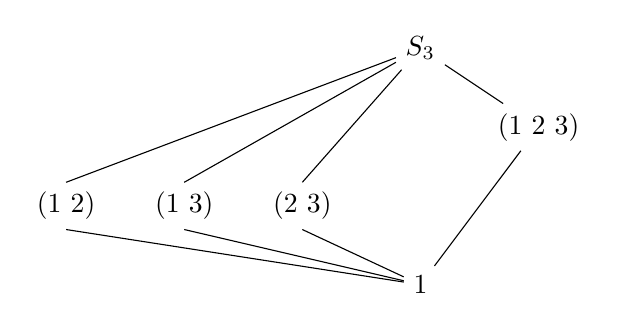
\begin{tikzpicture}
                \node (s3) at (0, 0) {$S_3$};
                \node (12) at (-4.5, -2) {$\gen{(1\ 2)}$};
                \node (13) at (-3, -2) {$\gen{(1\ 3)}$};
                \node (23) at (-1.5, -2) {$\gen{(2\ 3)}$};
                \node (123) at (1.5, -1) {$\gen{(1\ 2\ 3)}$};
                \node (1) at (0, -3) {1};

                \draw (1) -- (12.south);
                \draw (12.north) -- (s3);
                \draw (1) -- (13.south);
                \draw (13.north) -- (s3);
                \draw (1) -- (23.south);
                \draw (23.north) -- (s3);
                \draw (1) -- (123) -- (s3);
            \end{tikzpicture}
        \end{center}
        \begin{multicols}{2}
            \item $D_8$ is the lattice:
            \begin{center}
                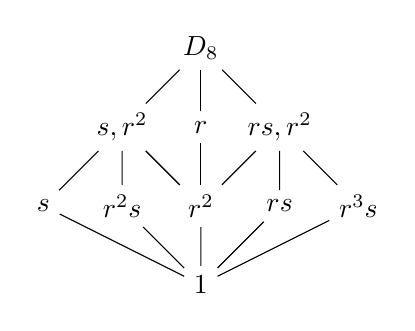
\begin{tikzpicture}
                    \node (d8) at (0, 0) {$D_8$};
                    \node (sr2) at (-1, -1) {$\gen{s, r^2}$};
                    \node (r) at (0, -1) {$\gen r$};
                    \node (rsr2) at (1, -1) {$\gen{rs, r^2}$};
                    \node (s) at (-2, -2) {$\gen s$};
                    \node (r2s) at (-1, -2) {$\gen{r^2s}$};
                    \node (r2) at (0, -2) {$\gen{r^2}$};
                    \node (rs) at (1, -2) {$\gen{rs}$};
                    \node (r3s) at (2, -2) {$\gen{r^3s}$};
                    \node (1) at (0, -3) {1};
    
                    \draw (1) -- (s) -- (sr2) -- (d8);
                    \draw (1) -- (r2s) -- (sr2);
                    \draw (1) -- (r2) -- (sr2);
                    \draw (1) -- (rs) -- (rsr2) -- (d8);
                    \draw (1) -- (r3s) -- (rsr2);
                    \draw (r2) -- (r) -- (d8);
                    \draw (r2) -- (sr2);
                    \draw (r2) -- (rsr2);
                \end{tikzpicture}
            \end{center}
            \item $Q_8$ is the lattice:
            \begin{center}
                \begin{tikzpicture}
                    \node (q8) at (0, 0) {$Q_8$};
                    \node (i) at (-1, -1) {$\gen i$};
                    \node (j) at (0, -1) {$\gen j$};
                    \node (k) at (1, -1) {$\gen k$};
                    \node (-1) at (0, -2) {$\gen{-1}$};
                    \node (1) at (0, -3) {1};
    
                    \draw (1) -- (-1) -- (i) -- (q8);
                    \draw (-1) -- (j) -- (q8);
                    \draw (-1) -- (k) -- (q8);
                \end{tikzpicture}
            \end{center}
        \end{multicols}
        \item $D_{16}$ has a lattice that is not a planar graph, or is a graph drawn on a plane without lines crossing. A way of drawing it is
        \begin{center}
            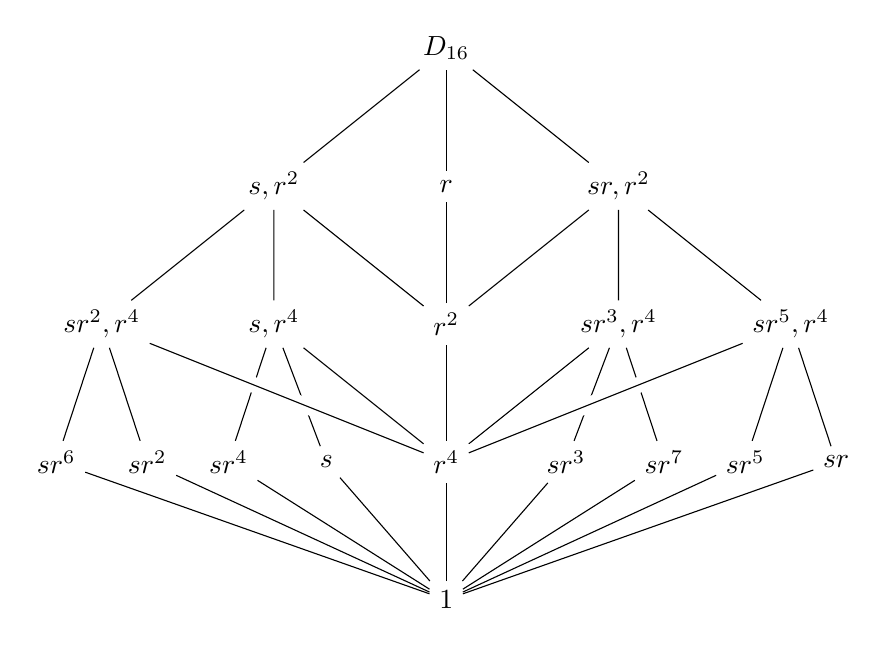
\begin{tikzpicture}[scale=1.75]
                \node (d16) at (0, 0) {$D_{16}$};

                \node (s r2) at (-1.25, -1) {$\gen{s, r^2}$};
                \node (r) at (0, -1) {$\gen r$};
                \node (srr2) at (1.25, -1) {$\gen{sr, r^2}$};

                \node (sr2r4) at (-2.5, -2) {$\gen{sr^2, r^4}$};
                \node (s r4) at (-1.25, -2) {$\gen{s, r^4}$};
                \node (r2) at (0, -2) {$\gen{r^2}$};
                \node (sr3r4) at (1.25, -2) {$\gen{sr^3, r^4}$};
                \node (sr5r4) at (2.5, -2) {$\gen{sr^5, r^4}$};

                \node (sr6) at (-2.83, -3) {$\gen{sr^6}$};
                \node (sr2) at (-2.17, -3) {$\gen{sr^2}$};
                \node (sr4) at (-1.58, -3) {$\gen{sr^4}$};
                \node (s) at (-0.87, -3) {$\gen s$};
                \node (r4) at (0, -3) {$\gen{r^4}$};
                \node (sr3) at (0.87, -3) {$\gen{sr^3}$};
                \node (sr7) at (1.58, -3) {$\gen{sr^7}$};
                \node (sr5) at (2.17, -3) {$\gen{sr^5}$};
                \node (sr) at (2.83, -3) {$\gen{sr}$};

                \node (1) at (0, -4) {1};

                \draw (1) -- (sr6) -- (sr2r4) -- (s r2) -- (d16);
                \draw (1) -- (sr2) -- (sr2r4);
                \draw (1) -- (sr4) -- (s r4) -- (s r2);
                \draw (1) -- (s) -- (s r4);
                \draw (1) -- (r4) -- (r2) -- (r) -- (d16);
                \draw (1) -- (sr3) -- (sr3r4) -- (srr2) -- (d16);
                \draw (1) -- (sr7) -- (sr3r4);
                \draw (1) -- (sr5) -- (sr5r4) -- (srr2);
                \draw (1) -- (sr) -- (sr5r4);
                \draw [preaction={draw, line width=2mm, white}] (r4) -- (sr2r4);
                \draw (r4) -- (s r4);
                \draw (r4) -- (sr3r4);
                \draw [preaction={draw, line width=2mm, white}] (r4) -- (sr5r4);
                \draw (r2) -- (s r2);
                \draw (r2) -- (srr2);
            \end{tikzpicture}
        \end{center}
    \end{enumerate}
\end{ex}

\begin{note}[Sublattices and Computing Centralizers and Normalizers]
    \begin{itemize}
        \item For any given proof or problem, we are often interested only in a portion of its subgroup lattice. We may then construct a \textit{sublattice} of the subgroup lattice, which involves only relevant joins and intersections for the groups. For example, we may discuss only the relationship between the subgroups $\gen{sr^2, r^4}$ and $\gen{r^2}$ of $D_{16}$, in which case we may draw the sublattice
        \begin{center}
            \begin{tikzpicture}
                \node (d16) at (0, 0) {$D_{16}$};
                \node (sr2) at (0, -1) {$\gen{s, r^2}$};
                \node (sr2r4) at (-1, -2) {$\gen{sr^2, r^4}$};
                \node (r2) at (1, -2) {$\gen{r^2}$};
                \node (r4) at (0, -3) {$\gen{r^4}$};
                \node (1) at (0, -4) {1};

                \draw (1) -- (r4) -- (sr2r4) -- (sr2) -- (d16);
                \draw (r4) -- (r2) -- (sr2);
            \end{tikzpicture}
        \end{center}
        \item When we have access to the subgroup lattice of a group, we can compute normalizers and centralizers. In $D_8$, we see that $C_{D_8}(s) = \gen{s, r^2}$ because we know that $r^2 \in C_{D_8}(s)$ so that $\gen{s, r^2} \leq C_{D_8}(s)$. Since no other subgroups that contain $\gen{s, r^2}$ except itself and $D_8$, and $r \not\in C_{D_8}(s)$ so that $C_{D_8}(s) \neq D_8$, it must be that $C_{D_8}(s) = \gen{s, r^2}$.
    \end{itemize}
\end{note}